\documentclass[11pt,letterpaper]{article}
\usepackage[lmargin=1in,rmargin=1in,tmargin=1in,bmargin=1in]{geometry}
\usepackage{../style/homework}
\usepackage{../style/commands}
\setbool{quotetype}{true} % True: Side; False: Under
\setbool{hideans}{true} % Student: True; Instructor: False

% -------------------
% Content
% -------------------
\begin{document}

\homework{10: Due 01/20}{I'm fast. To give you a reference point, I'm somewhere between a snake and a mongoose\dots and a panther.}{Dwight Schrute, The Office}

% Problem 1
\problem{10} Sketch the function $y= 10 \left( \dfrac{1}{2} \right)^x$. 
	\[
	\fbox{
	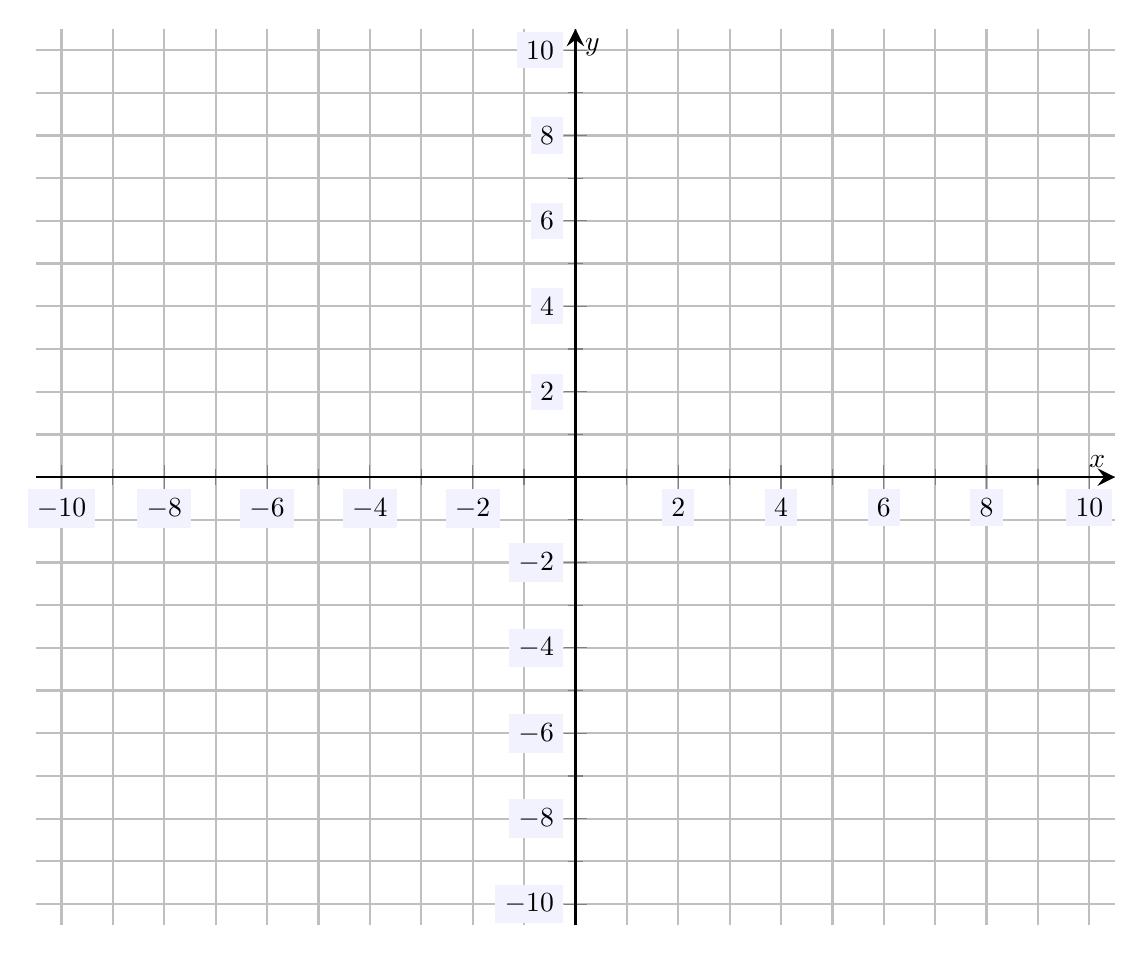
\begin{tikzpicture}[scale=2,every node/.style={scale=0.5}]
	\begin{axis}[
	grid=both,
	axis lines=middle,
	ticklabel style={fill=blue!5!white},
	xmin= -10.5, xmax=10.5,
	ymin= -10.5, ymax=10.5,
	xtick={-10,-8,-6,-4,-2,0,2,4,6,8,10},
	ytick={-10,-8,-6,-4,-2,0,2,4,6,8,10},
	minor tick = {-10,-9,...,10},
	xlabel=\(x\),ylabel=\(y\),
	]
	\end{axis}
	\end{tikzpicture}
	}
	\]



\newpage



% Problem 2
\problem{10} Sketch the function $y= 5 - 2^{1 - x}$.
	\[
	\fbox{
	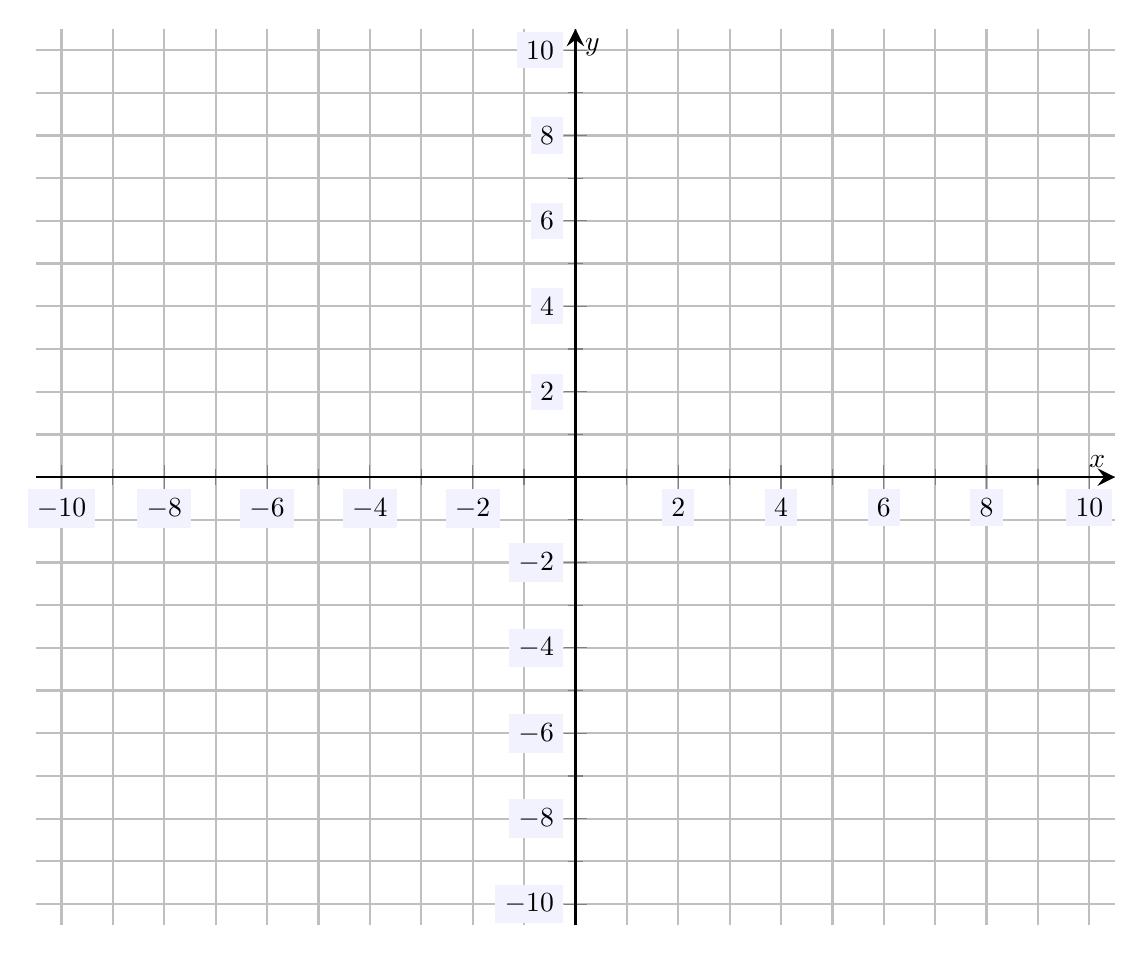
\begin{tikzpicture}[scale=2,every node/.style={scale=0.5}]
	\begin{axis}[
	grid=both,
	axis lines=middle,
	ticklabel style={fill=blue!5!white},
	xmin= -10.5, xmax=10.5,
	ymin= -10.5, ymax=10.5,
	xtick={-10,-8,-6,-4,-2,0,2,4,6,8,10},
	ytick={-10,-8,-6,-4,-2,0,2,4,6,8,10},
	minor tick = {-10,-9,...,10},
	xlabel=\(x\),ylabel=\(y\),
	]
	\end{axis}
	\end{tikzpicture}
	}
	\]



\newpage



% Problem 3
\problem{10} Write function $f(x)=  2 \left( \dfrac{1}{3} \right)^{2 - x}$ in the form $f(x)= Ab^x$, identifying $A$ and $b$, and determine whether the function $f(x)$ is increasing or decreasing. 



\newpage



% Problem 4
\problem{10} Write function $f(x)=  -5 \left( \dfrac{1}{3} \right)^{2 - x}$ in the form $f(x)= Ab^x$, identifying $A$ and $b$, and determine whether the function $f(x)$ is increasing or decreasing. 



\newpage



% Problem 5
\problem{10} Write function $f(x)=  6 - 2^{1 - 2x}$ in the form $f(x)= Ab^x + C$, identifying $A$, $b$, and $C$, and determine whether the function $f(x)$ is increasing or decreasing. 



\newpage



% Problem 6
\problem{10} Consider the function $y= -25 (5^{-3x})$.
        \begin{enumerate}[(a)]
        \item Is the function increasing or decreasing? Explain.
        \item Find the $y$-intercept of this function.
        \item What are the $x$-intercepts and zeros for this function?
        \item Find $y(-1)$. 
        \end{enumerate} 



\newpage



% Problem 7
\problem{10} Showing all your work, solve the following equation:
	\[
	3^{1 - x}= 27
	\]



\newpage



% Problem 8
\problem{10} Showing all your work, solve the following equation:
	\[
	64^x= \dfrac{1}{2}
	\]



\newpage



% Problem 9
\problem{10} Showing all your work, solve the following equation:
	\[
	2\left( \dfrac{1}{3} \right)^{-x} - 59= -5
	\]



\newpage



% Problem 10
\problem{10} Showing all your work, solve the following equation:
	\[
	2^{3x} - 7= 9
	\]


\end{document}